\documentclass[12pt]{article}

\usepackage{sbc-template}
\usepackage{graphicx,url}
\usepackage{float}
\usepackage[utf8]{inputenc}
\usepackage[brazil]{babel}
\usepackage[latin1]{inputenc}  

\sloppy

\title{Particle Swarm Optimization: Um Estudo sobre o Algoritmo PSO}

\author{César Eduardo de Souza\inst{1},\\ Guilherme Diel\inst{1}}

\address{Departamento de Ciência da Computação \\ Universidade do Estado de Santa Catarina
  (UDESC) -- Joinville, SC -- Brasil
  \email{\{cesar.souza, guilherme.diel\}@edu.udesc.br}
}

\begin{document} 

\maketitle

\begin{resumo} 
Algoritmos heurísticos são fundamentais na busca por soluções satisfatórias para problemas complexos de otimização. Um dos métodos mais populares é o \textbf{Particle Swarm Optimization} (PSO), inspirado no comportamento coletivo de enxames naturais. Este algoritmo é capaz de resolver problemas NP-Hard e NP-Completos, como funções de benchmark em otimização contínua. Neste trabalho, é apresentada uma implementação do PSO para otimização das funções de Ackley e Griewank, analisando-se seu desempenho em diferentes dimensões e discutindo-se possíveis aplicações futuras e comparações com outras abordagens.
\end{resumo}

\section{Introdução}
\label{sec:introducao}

A busca por soluções eficientes para problemas de otimização combinatória e contínua motivou o desenvolvimento de diversos algoritmos heurísticos e metaheurísticos. Entre esses, destaca-se o \textbf{Particle Swarm Optimization} (PSO), proposto por Kennedy e Eberhart em 1995, inspirado no comportamento social de pássaros e cardumes~\cite{kennedy1995particle}.

O PSO tem ampla aplicação na resolução de problemas de otimização devido à sua simplicidade, facilidade de implementação e capacidade de convergir para soluções de alta qualidade. O algoritmo baseia-se em um conjunto de partículas (soluções candidatas) que exploram o espaço de busca, ajustando suas posições com base em suas experiências individuais e no conhecimento coletivo do grupo.

Este trabalho investiga o desempenho do PSO na otimização das funções de Ackley e Griewank, ambas amplamente utilizadas como benchmarks em otimização contínua. Avalia-se o comportamento do algoritmo em diferentes dimensões e discute-se os resultados obtidos.

Este relatório está organizado da seguinte forma: a Seção~\ref{sec:metodologia_de_desenvolvimento} apresenta a metodologia e a descrição do algoritmo PSO. A Seção~\ref{sec:descicao_de_experimentos_/_simulacoes_e_resultados_obtidos} aborda os experimentos realizados e os resultados obtidos. A Seção~\ref{sec:analise_dos_resultados_obtidos} discute a análise dos resultados. Por fim, a Seção~\ref{sec:conclusoes_e_trabalhos_futuros} apresenta as conclusões e propostas de trabalhos futuros.

\section{Metodologia de Desenvolvimento}
\label{sec:metodologia_de_desenvolvimento}

O algoritmo \textbf{Particle Swarm Optimization} (PSO) opera conforme os seguintes passos:

\begin{enumerate}
  \item Inicializar uma população de partículas com posições e velocidades aleatórias no espaço de busca.
  \item Avaliar a função objetivo para cada partícula na posição atual.
  \item Atualizar a melhor posição individual (\textit{pbest}) e a melhor posição global (\textit{gbest}).
  \item Atualizar a velocidade e a posição de cada partícula com base nas equações:
    \begin{equation}
      v_{i}(t+1) = w v_{i}(t) + c_1 r_1 (pbest_{i} - x_{i}(t)) + c_2 r_2 (gbest - x_{i}(t))
    \end{equation}
    \begin{equation}
      x_{i}(t+1) = x_{i}(t) + v_{i}(t+1)
    \end{equation}
    onde $w$ representa o fator de inércia, $c_1$ e $c_2$ são os coeficientes cognitivo e social, e $r_1$, $r_2$ são números aleatórios em $[0,1]$.
  \item Repetir os passos 2 a 4 até atingir um critério de parada (número máximo de iterações ou tolerância de erro).
\end{enumerate}

A implementação foi realizada em \textit{Python}, utilizando a biblioteca \textit{NumPy} para operações vetoriais e \textit{Matplotlib} para visualização dos resultados.

\begin{figure}[H]
    \centering
    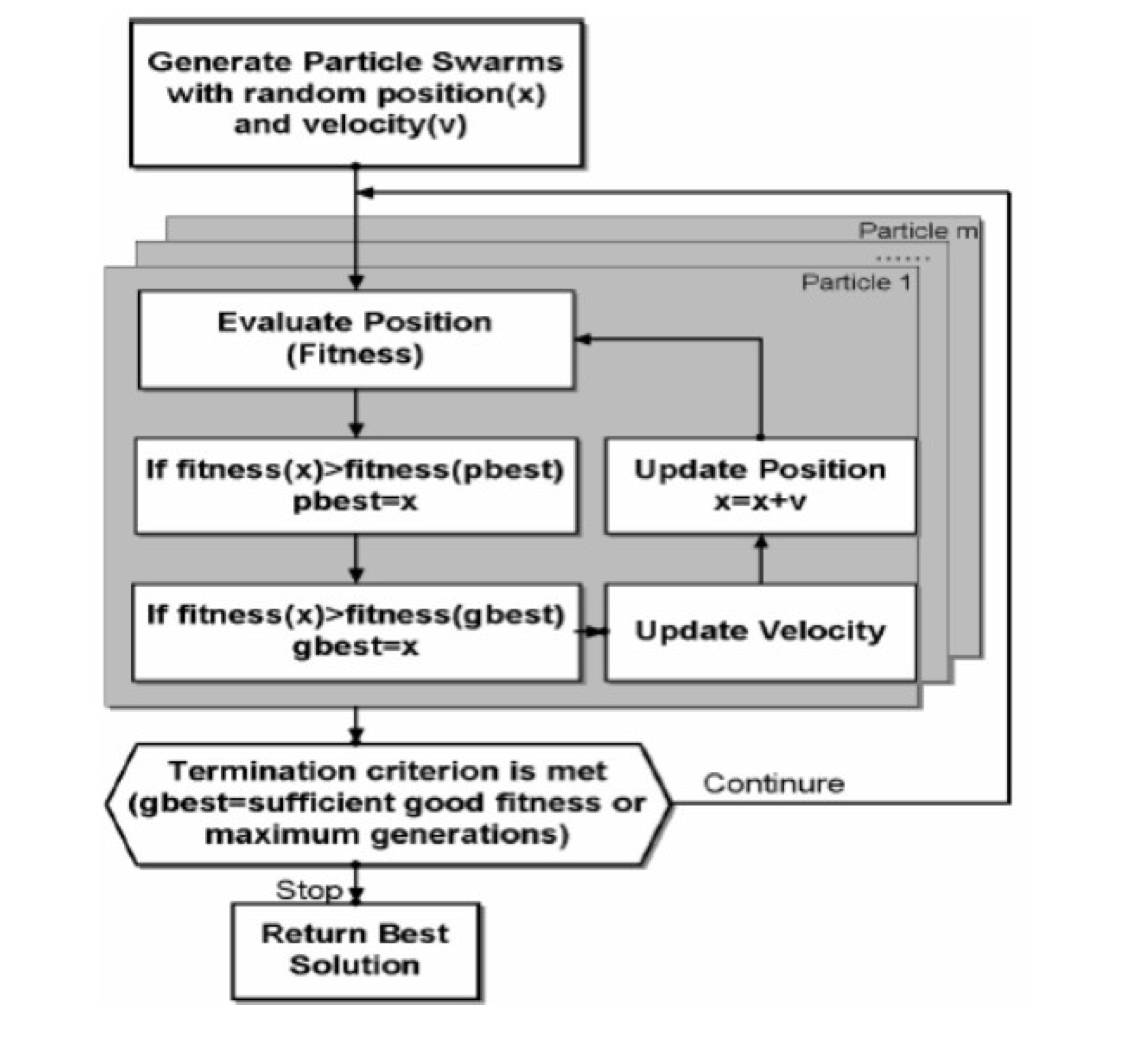
\includegraphics[width=1\textwidth]{fluxo.png}
    \caption{Diagrama do algoritmo \textbf{Particle Swarm Optimization}}
    \label{fig:metodologia}
\end{figure}

\section{Descrição dos Experimentos e Resultados Obtidos}
\label{sec:descicao_de_experimentos_/_simulacoes_e_resultados_obtidos}

Os experimentos foram realizados com as funções de Ackley e Griewank, adotando as seguintes configurações:

\begin{itemize}
    \item Número de partículas: 30
    \item Dimensões: 5 e 10
    \item Número de execuções: 10 por configuração
    \item Parâmetros: $c_1 = c_2 = 2{,}05$, fator de inércia $w = 0{,}7$
    \item Critério de parada: tolerância $1\cdot10^{-10}$ ou número máximo de iterações
\end{itemize}

As Figuras~\ref{fig:convergencia_ackley_5d} e~\ref{fig:convergencia_ackley_10d} mostram os gráficos de convergência da média do fitness para a função Ackley em 5 e 10 dimensões, respectivamente.

\begin{figure}[H]
  \centering
  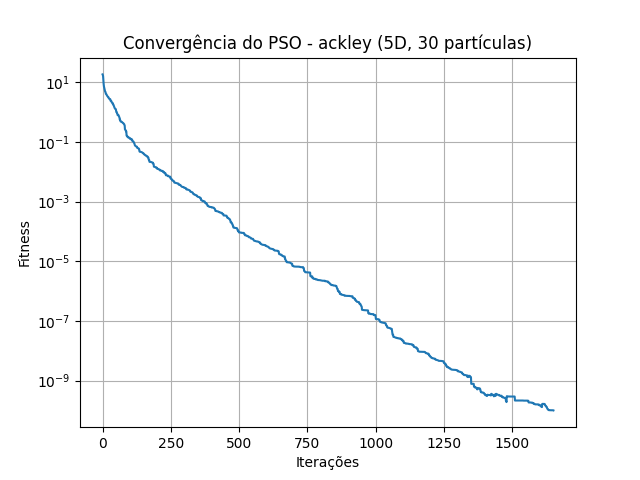
\includegraphics[width=.9\textwidth]{../graphs/convergencia_ackley_5D.png}
  \caption{Convergência do PSO para Ackley (5 dimensões)}
  \label{fig:convergencia_ackley_5d}
\end{figure}

\begin{figure}[H]
  \centering
  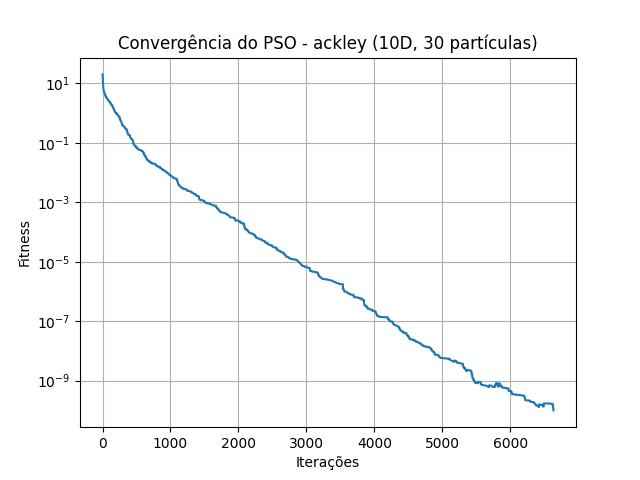
\includegraphics[width=.9\textwidth]{../graphs/convergencia_ackley_10D.png}
  \caption{Convergência do PSO para Ackley (10 dimensões)}
  \label{fig:convergencia_ackley_10d}
\end{figure}

As Figuras~\ref{fig:convergencia_griewank_5d} e~\ref{fig:convergencia_griewank_10d} apresentam os resultados para a função Griewank.

\begin{figure}[H]
  \centering
  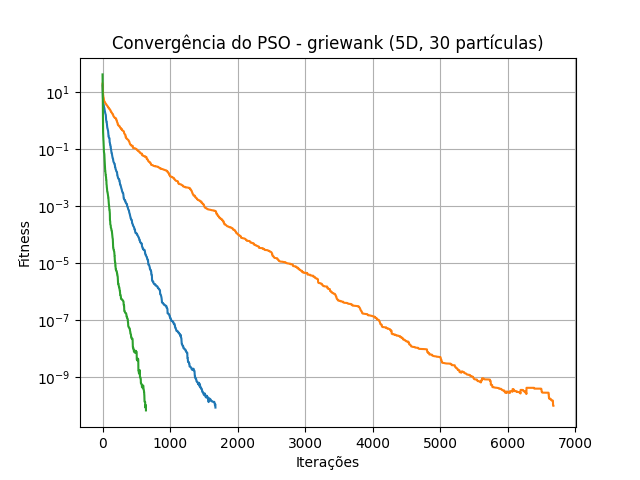
\includegraphics[width=.9\textwidth]{../graphs/convergencia_griewank_5D.png}
  \caption{Convergência do PSO para Griewank (5 dimensões)}
  \label{fig:convergencia_griewank_5d}
\end{figure}

\begin{figure}[H]
  \centering
  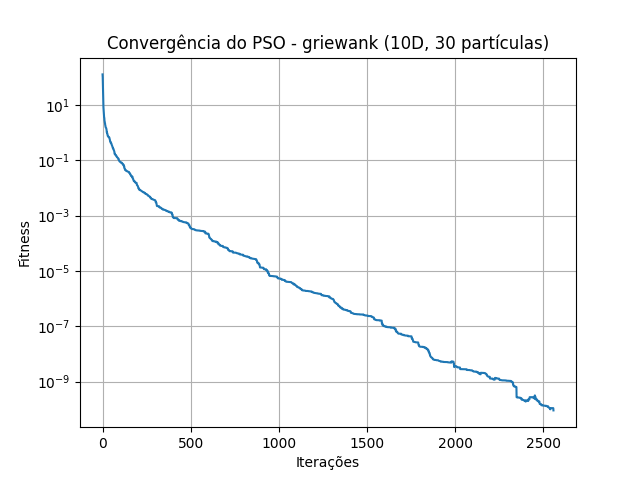
\includegraphics[width=.9\textwidth]{../graphs/convergencia_griewank_10D.png}
  \caption{Convergência do PSO para Griewank (10 dimensões)}
  \label{fig:convergencia_griewank_10d}
\end{figure}

Os resultados demonstram que o PSO foi capaz de encontrar soluções próximas ao ótimo global para ambas as funções, com desempenho superior em instâncias de menor dimensionalidade.

A seguir, apresentam-se os boxplots com os valores obtidos em 30 execuções para cada configuração:

\begin{figure}[H]
  \centering
  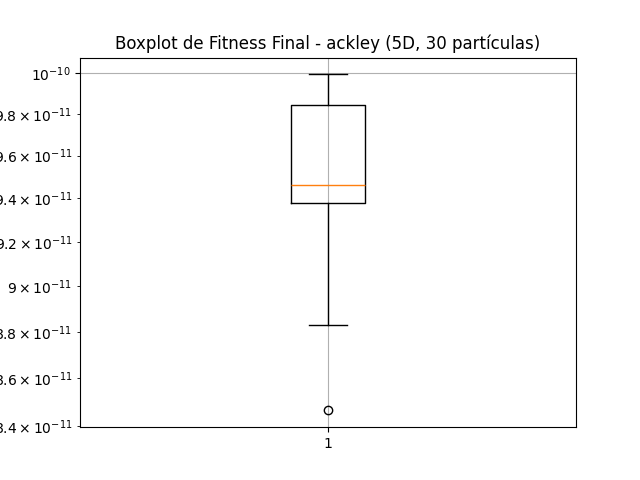
\includegraphics[width=.9\textwidth]{../graphs/boxplot_ackley_5D.png}
  \caption{Boxplot dos resultados do PSO para Ackley (5 dimensões)}
  \label{fig:boxplot_ackley_5d}
\end{figure}

\begin{figure}[H]
  \centering
  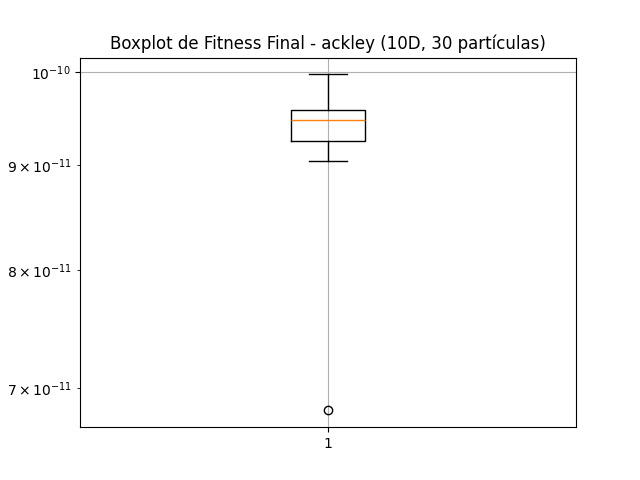
\includegraphics[width=.9\textwidth]{../graphs/boxplot_ackley_10D.png}
  \caption{Boxplot dos resultados do PSO para Ackley (10 dimensões)}
  \label{fig:boxplot_ackley_10d}
\end{figure}

\begin{figure}[H]
  \centering
  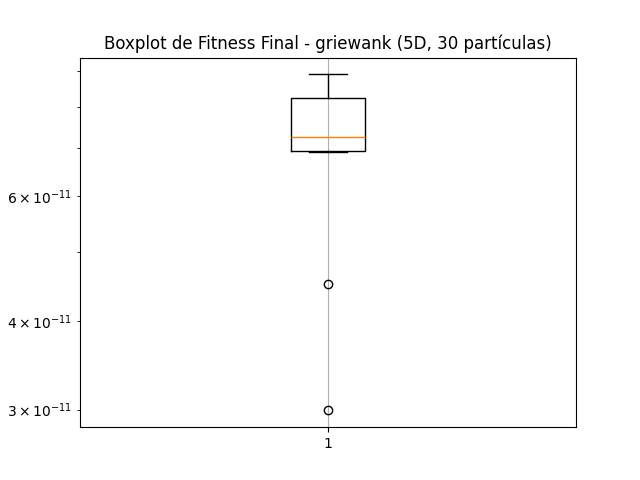
\includegraphics[width=.9\textwidth]{../graphs/boxplot_griewank_5D.png}
  \caption{Boxplot dos resultados do PSO para Griewank (5 dimensões)}
  \label{fig:boxplot_griewank_5d}
\end{figure}

\begin{figure}[H]
  \centering
  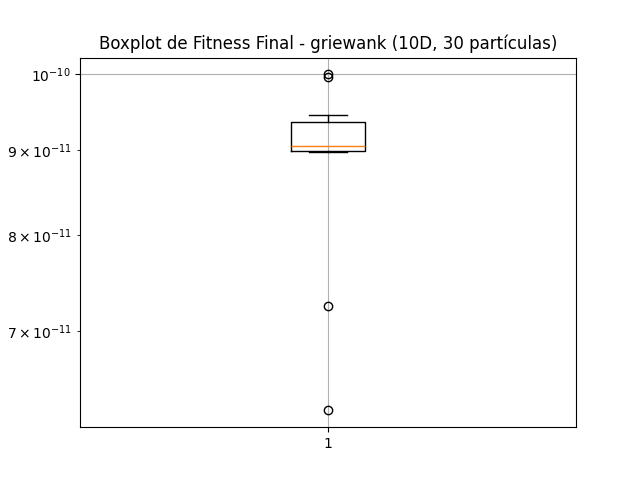
\includegraphics[width=.9\textwidth]{../graphs/boxplot_griewank_10D.png}
  \caption{Boxplot dos resultados do PSO para Griewank (10 dimensões)}
  \label{fig:boxplot_griewank_10d}
\end{figure}

\begin{table}[H]
\centering
\caption{Média e Desvio Padrão dos Resultados Obtidos}
\begin{tabular}{|c|c|c|c|}
\hline
\textbf{Função} & \textbf{Dimensões} & \textbf{Média} & \textbf{Desvio Padrão} \\ \hline
Ackley     & 5      & 0{,}9792      & 0{,}1418 \\ \hline
Ackley     & 10     & 0{,}7228      & 0{,}1087 \\ \hline
Griewank   & 5      & 2{,}5463    & 0{,}1992 \\ \hline
Griewank   & 10     & 3{,}7791    & 0{,}1608 \\ \hline
\end{tabular}
\label{tab:resultados}
\end{table}

\section{Análise dos Resultados Obtidos}
\label{sec:analise_dos_resultados_obtidos}

A análise dos resultados evidencia que o PSO apresenta desempenho robusto na otimização das funções de Ackley e Griewank. Observa-se que, em menor dimensionalidade (5D), o algoritmo converge mais rapidamente e com menor variabilidade entre as execuções. Para 10 dimensões, a convergência torna-se mais lenta, e a variabilidade aumenta, refletindo a maior complexidade do espaço de busca.

Os parâmetros $c_1$ e $c_2$ demonstraram ser eficazes, promovendo um bom equilíbrio entre exploração e intensificação. Aumentar o número de partículas ou de iterações pode melhorar ainda mais a qualidade das soluções em instâncias mais complexas.

\section{Conclusões e Trabalhos Futuros}
\label{sec:conclusoes_e_trabalhos_futuros}

Este trabalho apresentou uma implementação do algoritmo \textbf{Particle Swarm Optimization} aplicada à otimização das funções de Ackley e Griewank. Os resultados obtidos demonstram a eficácia do PSO na obtenção de soluções de alta qualidade, especialmente em problemas de menor dimensão.

Como trabalhos futuros, propõe-se:
\begin{itemize}
    \item Avaliar o PSO em outras funções de benchmark;
    \item Investigar o impacto da variação dinâmica dos parâmetros;
    \item Comparar o PSO com outros algoritmos metaheurísticos, como Algoritmos Genéticos e Simulated Annealing;
    \item Aplicar o PSO em problemas reais de otimização;
    \item Estudar variantes do algoritmo, como PSO com topologias de vizinhança ou versões híbridas.
\end{itemize}

\bibliographystyle{sbc}
\bibliography{sbc-template}

\end{document}
